\section{SORA Payload Description}
\label{sec:Hardware}

%Subsections:
%Talk about general design of each component or payload part.  Go into detail about choice of materials, placement, and reasoning for the success of the mission.  Also, try to include either real photos, CAD designs or any other relevant graphic.  
%\subsection{MiniPIX}
%MiniPIX
%\subsection{Flight Computer and Sensors}
%Flight Computer and Sensors (include the electric schematics)
%\subsection{Astrobiology}
%Astrobiology (lots of CAD designs)
%\subsection{Payload Structure and Outer Shell}
%Outer Shell (CAD designs and choice of materials)
%Notes:
%Outer material is Kydex from McMasterCarr
%Part PVC and part acrylic
%Manufacturer Specs:
%	https://www.mcmaster.com/acrylic/pvc
%	hydrophobic
%	UV resistant - no sun deterioration
%	3/16 inch thick
%	Color - white
%	Temperature range from -40 F to 150 F
%	Tensile Strength of 6,100 psi
%	Impact strength 15.00 ft.-lbs./in 
%	UL 94V0
%Commonly used for vehicle interiors and equipment housings, this material maintains its shape after heating and forming. It is also known as Kydex. These sheets resist corrosive chemicals and cleaning solutions. One side is smooth; the other side is coarse to mask scratches, scuffs, and fingerprints.
%
%Coated iron bolts, standard size for heavy mounting options
%Nickle plated L-brackets and brackets for wall mounting
%Machine cut to specifications (will include a figure here with all the dimensions)
%\begin{figure}[h!]
%	\begin{center}
%		\includegraphics[width=\textwidth]{figures/[figure name here]}
%		\caption{Payload Final Design}
%		\label{fig:payload_design}
%	\end{center}
%\end{figure}
%
%\begin{figure}[h!]
%	\begin{center}
%		\includegraphics[width=\textwidth]{figures/[figure name here]}
%		\caption{Picture of payload mounted onto gondola}
%		\label{fig:payload_gondola}
%	\end{center}
%\end{figure}

\begin{figure}[h!]
	\begin{center}
		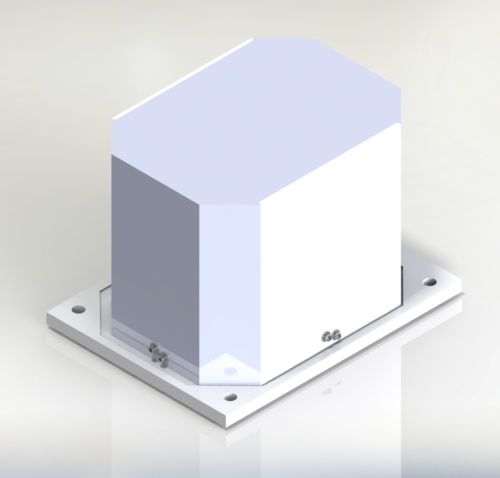
\includegraphics[width=50 mm, scale=0.7]{figures/payload_render.pdf}
		\caption{Payload Final Design}
		\label{fig:payload_render}
	\end{center}
\end{figure}
